
%(BEGIN_QUESTION)
% Copyright 2006, Tony R. Kuphaldt, released under the Creative Commons Attribution License (v 1.0)
% This means you may do almost anything with this work of mine, so long as you give me proper credit

A tank expert system gives the following pressure indications from its three transmitters:

$$\includegraphics[width=15.5cm]{i00255x01.eps}$$

From these pressure measurements, determine the level of liquid in the vessel and its specific gravity.  Be sure to explain how you obtained your answers!

\underbar{file i00255}
%(END_QUESTION)





%(BEGIN_ANSWER)

The ``Top'' transmitter's indication of 0 inches water column tells us that the vessel is vented, or at least there is no vapor pressure buildup in it.  This makes the task of determining level and density from the other two pressure measurements that much easier.

Determining specific gravity would be the best step to do first, before trying to determine liquid level.  Once the liquid's density is known, its level may be easily calculated from the ``Bottom'' transmitter's pressure measurement.

With 10 feet of vertical distance separating the ``Bottom'' and ``Middle'' transmitters, there should be 120 inches (10 feet $\times$ 12 inches/foot) of water column pressure {\it difference} between the two transmitters' measurements if the liquid in question had a specific gravity equal to 1, like water.  In this case, though, there is a pressure difference of only 110.4 inches between the two measurements:

\vskip 10pt

(276 "W.C.) - (165.6 "W.C.) = 110.4 "W.C.

\vskip 10pt

The discrepancy between 120 inches water column and 110.4 inches water column is due to one factor and one factor only: the liquid's density.  We may find the density by dividing the actual pressure difference by the expected pressure difference assuming a density equal to water:

\vskip 10pt

Specific gravity = (110.4 "W.C. / 120 "W.C.) = 0.92

\vskip 10pt

Therefore, the liquid held in this vessel has a specific gravity of 0.92, meaning that its density is 92\% that of water.  Knowing the liquid density, we calculate the liquid level by re-working the liquid column pressure equation to solve for height:

$$P = hG$$

$${P \over G} = h$$

\noindent
Where,

$P$ = hydrostatic pressure in inches water column

$h$ = liquid column height in inches

$G$ = specific gravity of liquid

\vskip 10pt

(276 "W.C.)/(0.92 "W.C. / in) = 300 inches

\vskip 10pt

So, the answer for liquid level is 300 inches, or 25 feet.

%(END_ANSWER)





%(BEGIN_NOTES)


%INDEX% Measurement, level: hydrostatic pressure
%INDEX% Measurement, level: tank expert system

%(END_NOTES)


